% answers.tex —— 2011 年·福建卷·理科 · 参考答案与详细解析片段
% 由 tools/generate_projects.py 依来源总账自 2011/2011_数学真题_福建理_试题.md + 2011/2011_数学真题_福建理_解析正文.md + 2011/2011_数学真题_福建理_答案要点.md 生成，勿手改（改源 MD 后重跑）

\begin{answer}
\gksolhead{1}{}

\textbf{题目}：

$\mathrm i$ 是虚数单位，若集合 $S=\{-1,0,1\}$，则\mbox{（　　）}

（A）$\mathrm i\in S$

（B）$\mathrm i^2\in S$

（C）$\mathrm i^3\in S$

（D）$\dfrac2{\mathrm i}\in S$

\Needspace{4\baselineskip}
\textbf{解析}
$\mathrm i^2=-1\in S$。选 B。

\gkanswer{答案：B。}

\end{answer}
\begin{answer}
\gksolhead{2}{}

\textbf{题目}：

若 $a\in\mathbf R$，则“$a=2$”是“$(a-1)(a-2)=0$”的\mbox{（　　）}

（A）充分而不必要条件

（B）必要而不充分条件

（C）充要条件

（D）既不充分也不必要条件

\Needspace{4\baselineskip}
\textbf{解析}
$a=2$ 使 $(a-1)(a-2)=0$；反之 $a=1$ 也满足，故充分不必要。选 A。

\gkanswer{答案：A。}

\end{answer}
\begin{answer}
\gksolhead{3}{}

\textbf{题目}：

若 $\tan\alpha=3$，则 $\dfrac{\sin2\alpha}{\cos^2\alpha}$ 的值等于\mbox{（　　）}

（A）$2$

（B）$3$

（C）$4$

（D）$6$

\Needspace{4\baselineskip}
\textbf{解析}
\nopagebreak[4]
\[\frac{\sin2\alpha}{\cos^2\alpha}=\frac{2\sin\alpha\cos\alpha}{\cos^2\alpha}=2\tan\alpha=6.\]
选 D。

\gkanswer{答案：D。}

\end{answer}
\begin{answer}
\gksolhead{4}{}

\textbf{题目}：

如图，矩形 $ABCD$ 中，点 $E$ 为边 $CD$ 的中点，若在矩形 $ABCD$ 内部随机取一个点 $Q$，则点 $Q$ 取自 $\triangle ABE$ 内部的概率等于\mbox{（　　）}

（A）$\dfrac14$

（B）$\dfrac13$

（C）$\dfrac12$

（D）$\dfrac23$
\nopagebreak[4]
\begin{center}% 2011 年福建卷理科第 4 题：矩形与三角形 ABE。
% 来源 PDF：普通高考/2011/2011福建理.pdf，SHA-256 1a36c388b64669b29d16fe359efb087d96026059df01d26759f8bb5dd48342f1。
% 原页：第 1 页第 1 栏中部，书页码 659。
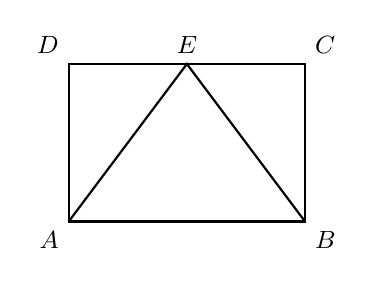
\begin{tikzpicture}[>=stealth, semithick, font=\small, scale=1.0]
  \coordinate (A) at (0,0);
  \coordinate (B) at (3,0);
  \coordinate (C) at (3,2);
  \coordinate (D) at (0,2);
  \coordinate (E) at (1.5,2);
  \draw[thick] (A)--(B)--(C)--(D)--cycle;
  \draw[thick] (A)--(E)--(B);
  \node[below left] at (A) {$A$};
  \node[below right] at (B) {$B$};
  \node[above right] at (C) {$C$};
  \node[above left] at (D) {$D$};
  \node[above] at (E) {$E$};
\end{tikzpicture}
\end{center}
\nopagebreak[4]
\Needspace{4\baselineskip}
\textbf{解析}
$\triangle ABE$ 的底 $AB$ 与矩形相同，高等于矩形的宽，故面积为矩形的一半，概率 $\dfrac12$。选 C。

\gkanswer{答案：C。}

\end{answer}
\begin{answer}
\gksolhead{5}{}

\textbf{题目}：

$\displaystyle\int_0^1(\mathrm e^x+2x)\,\mathrm dx$ 等于\mbox{（　　）}

（A）$1$

（B）$\mathrm e-1$

（C）$\mathrm e$

（D）$\mathrm e+1$

\Needspace{4\baselineskip}
\textbf{解析}
\nopagebreak[4]
\[\int_0^1(\mathrm e^x+2x)\,\mathrm dx=\left[\mathrm e^x+x^2\right]_0^1=(\mathrm e+1)-1=\mathrm e.\]
选 C。

\gkanswer{答案：C。}

\end{answer}
\begin{answer}
\gksolhead{6}{}

\textbf{题目}：

$(1+2x)^5$ 的展开式中，$x^2$ 的系数等于\mbox{（　　）}

（A）$80$

（B）$40$

（C）$20$

（D）$10$

\Needspace{4\baselineskip}
\textbf{解析}
$x^2$ 项系数 $\mathrm C_5^2\cdot2^2=10\cdot4=40$。选 B。

\gkanswer{答案：B。}

\end{answer}
\begin{answer}
\gksolhead{7}{}

\textbf{题目}：

设圆锥曲线 $\Gamma$ 的两个焦点分别为 $F_1$，$F_2$。若曲线 $\Gamma$ 上存在点 $P$ 满足 $|PF_1|:|F_1F_2|:|PF_2|=4:3:2$，则曲线 $\Gamma$ 的离心率等于\mbox{（　　）}

（A）$\dfrac12$ 或 $\dfrac32$

（B）$\dfrac23$ 或 $2$

（C）$\dfrac12$ 或 $2$

（D）$\dfrac23$ 或 $\dfrac32$

\Needspace{4\baselineskip}
\textbf{解析}
三边之比 $4:3:2$，$2c$ 对应 $3$。若为椭圆，$2a=4+2=6$，$e=\dfrac{2c}{2a}=\dfrac36=\dfrac12$；若为双曲线，$2a=4-2=2$，$e=\dfrac32$。选 A。

\gkanswer{答案：A。}

\end{answer}
\begin{answer}
\gksolhead{8}{}

\textbf{题目}：

已知 $O$ 是坐标原点，点 $A(-1,1)$，若点 $M(x,y)$ 为平面区域 $\begin{cases}x+y\geqslant2,\\x\leqslant1,\\y\leqslant2\end{cases}$ 上的一个动点，则 $\overrightarrow{OA}\cdot\overrightarrow{OM}$ 的取值范围是\mbox{（　　）}

（A）$[-1,0]$

（B）$[0,1]$

（C）$[0,2]$

（D）$[-1,2]$

\Needspace{4\baselineskip}
\textbf{解析}
$\overrightarrow{OA}\cdot\overrightarrow{OM}=-x+y$。可行域顶点 $(1,1)$，$(0,2)$，$(1,2)$，对应值 $0,2,1$，故范围 $[0,2]$。选 C。

\gkanswer{答案：C。}

\end{answer}
\begin{answer}
\gksolhead{9}{}

\textbf{题目}：

对于函数 $f(x)=a\sin x+bx+c$（其中 $a$，$b\in\mathbf R$，$c\in\mathbf Z$），选取 $a$，$b$，$c$ 的一组值计算 $f(1)$ 和 $f(-1)$，所得出的正确结果一定不可能是\mbox{（　　）}

（A）$4$ 和 $6$

（B）$3$ 和 $1$

（C）$2$ 和 $4$

（D）$1$ 和 $2$

\Needspace{4\baselineskip}
\textbf{解析}
$f(1)+f(-1)=2c$ 为偶数，$f(1)-f(-1)=2(a\sin1+b)$。选项中（D）两数之和 $3$ 为奇数，不可能。选 D。

\gkanswer{答案：D。}

\end{answer}
\begin{answer}
\gksolhead{10}{}

\textbf{题目}：

已知函数 $f(x)=\mathrm e^x+x$，对于曲线 $y=f(x)$ 上横坐标成等差数列的三个点 $A$，$B$，$C$，给出以下判断：① $\triangle ABC$ 一定是钝角三角形；② $\triangle ABC$ 可能是直角三角形；③ $\triangle ABC$ 可能是等腰三角形；④ $\triangle ABC$ 不可能是等腰三角形。其中，正确的判断是\mbox{（　　）}

（A）①③

（B）①④

（C）②③

（D）②④

\Needspace{4\baselineskip}
\textbf{解析}
$f''(x)=\mathrm e^x>0$，曲线下凸。横坐标等差的三点中，中间点位于弦 $AC$ 下方，$\angle ABC$ 为钝角，①真、②假；又严格下凸使 $AB\ne BC$，且可证 $AB\ne AC$，故不可能为等腰三角形，④真。选 B。

\gkanswer{答案：B。}

\end{answer}
\begin{answer}
\gksolhead{11}{}

\textbf{题目}：

运行如图所示的程序，输出的结果是 $\underline{\qquad}$。
\nopagebreak[4]
\begin{center}% 2011 年福建卷理科第 11 题：伪代码。
% 来源 PDF：普通高考/2011/2011福建理.pdf，SHA-256 1a36c388b64669b29d16fe359efb087d96026059df01d26759f8bb5dd48342f1。
% 原页：第 1 页第 2 栏上部，书页码 659。
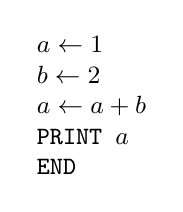
\begin{tikzpicture}[font=\ttfamily\small, semithick]
  \node[anchor=west, align=left] at (0,0) {%
    $a\leftarrow1$\\
    $b\leftarrow2$\\
    $a\leftarrow a+b$\\
    PRINT $a$\\
    END};
\end{tikzpicture}
\end{center}
\nopagebreak[4]
\Needspace{4\baselineskip}
\textbf{解析}
$a=1$，$b=2$，$a\leftarrow a+b=3$，输出 $3$。

\gkanswer{答案：$3$。}

\end{answer}
\begin{answer}
\gksolhead{12}{}

\textbf{题目}：

三棱锥 $P-ABC$ 中，$PA\perp$ 底面 $ABC$，$PA=3$，底面 $ABC$ 是边长为 $2$ 的正三角形，则三棱锥 $P-ABC$ 的体积等于 $\underline{\qquad}$。

\Needspace{4\baselineskip}
\textbf{解析}
\Needspace{5\baselineskip}
底面积 $\dfrac{\sqrt3}4\cdot2^2=\sqrt3$，高 $3$，体积
\nopagebreak[4]
\[V=\frac13\cdot\sqrt3\cdot3=\sqrt3.\]

\gkanswer{答案：$\sqrt3$。}

\end{answer}
\begin{answer}
\gksolhead{13}{}

\textbf{题目}：

盒中装有形状、大小完全相同的 $5$ 个球，其中红色球 $3$ 个，黄色球 $2$ 个。若从中随机取出 $2$ 个球，则所取出的 $2$ 个球颜色不同的概率等于 $\underline{\qquad}$。

\Needspace{4\baselineskip}
\textbf{解析}
\nopagebreak[4]
\[P=\frac{\mathrm C_3^1\mathrm C_2^1}{\mathrm C_5^2}=\frac6{10}=\frac35.\]

\gkanswer{答案：$\dfrac35$。}

\end{answer}
\begin{answer}
\gksolhead{14}{}

\textbf{题目}：

如图，$\triangle ABC$ 中，$AB=AC=2$，$BC=2\sqrt3$，点 $D$ 在 $BC$ 边上，$\angle ADC=45^\circ$，则 $AD$ 的长度等于 $\underline{\qquad}$。
\nopagebreak[4]
\begin{center}% 2011 年福建卷理科第 14 题：△ABC 与 BC 上一点 D。
% 来源 PDF：普通高考/2011/2011福建理.pdf，SHA-256 1a36c388b64669b29d16fe359efb087d96026059df01d26759f8bb5dd48342f1。
% 原页：第 1 页第 2 栏中部，书页码 659。
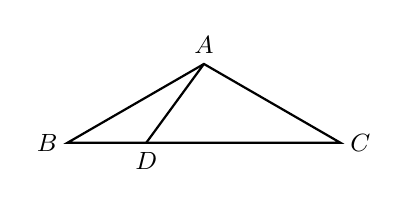
\begin{tikzpicture}[>=stealth, semithick, font=\small, scale=1.0]
  \coordinate (B) at (0,0);
  \coordinate (C) at (3.464,0);
  \coordinate (A) at (1.732,1.0);
  \coordinate (D) at (1.0,0);
  \draw[thick] (A)--(B)--(C)--cycle;
  \draw[thick] (A)--(D);
  \node[above] at (A) {$A$};
  \node[left] at (B) {$B$};
  \node[right] at (C) {$C$};
  \node[below] at (D) {$D$};
\end{tikzpicture}
\end{center}
\nopagebreak[4]
\Needspace{4\baselineskip}
\textbf{解析}
\Needspace{5\baselineskip}
$\cos A=\dfrac{4+4-12}{8}=-\dfrac12$，故 $A=120^\circ$，$B=C=30^\circ$。在 $\triangle ACD$ 中 $\angle ACD=30^\circ$，$\angle ADC=45^\circ$，故 $\angle CAD=105^\circ$。由正弦定理
\nopagebreak[4]
\[\frac{AD}{\sin30^\circ}=\frac{AC}{\sin45^\circ}\Longrightarrow AD=2\cdot\frac{1/2}{\sqrt2/2}=\sqrt2.\]

\gkanswer{答案：$\sqrt2$。}

\end{answer}
\begin{answer}
\gksolhead{15}{}

\textbf{题目}：

设 $V$ 是全体平面向量构成的集合，若映射 $f:V\to\mathbf R$ 满足：对任意向量 $\boldsymbol a=(x_1,y_1)\in V$，$\boldsymbol b=(x_2,y_2)\in V$，以及任意 $\lambda\in\mathbf R$，均有 $f(\lambda\boldsymbol a+(1-\lambda)\boldsymbol b)=\lambda f(\boldsymbol a)+(1-\lambda)f(\boldsymbol b)$，则称映射 $f$ 具有性质 $P$。现给出如下映射：① $f_1:V\to\mathbf R$，$f_1(\boldsymbol m)=x-y$，$\boldsymbol m=(x,y)\in V$；② $f_2:V\to\mathbf R$，$f_2(\boldsymbol m)=x^2+y$，$\boldsymbol m=(x,y)\in V$；③ $f_3:V\to\mathbf R$，$f_3(\boldsymbol m)=x+y+1$，$\boldsymbol m=(x,y)\in V$。其中，具有性质 $P$ 的映射的序号为 $\underline{\qquad}$。

\Needspace{4\baselineskip}
\textbf{解析}
性质 $P$ 即仿射线性。$f_1$ 为线性映射，满足；$f_2$ 含 $x^2$，不满足；$f_3=x+y+1$ 为仿射映射，且权重和为 $1$，满足。故填 ①③。

\gkanswer{答案：①③。}

\end{answer}
\begin{answer}
\gksolhead{16}{}

\textbf{题目}：

已知等比数列 $\{a_n\}$ 的公比 $q=3$，前 $3$ 项和 $S_3=\dfrac{13}3$。

（1） 求数列 $\{a_n\}$ 的通项公式；

（2） 若函数 $f(x)=A\sin(2x+\varphi)$（$A>0$，$0<\varphi<\pi$）在 $x=\dfrac\pi6$ 处取得最大值，且最大值为 $a_3$，求函数 $f(x)$ 的解析式。

\Needspace{4\baselineskip}
\textbf{解析}
\gksubpart{(1)}
$S_3=a_1(1+3+9)=13a_1=\dfrac{13}3$，故 $a_1=\dfrac13$，$a_n=\dfrac13\cdot3^{n-1}=3^{n-2}$。

\gksubpart{(2)}
\Needspace{5\baselineskip}
$a_3=3$。$x=\dfrac\pi6$ 处取最大值：$2\cdot\dfrac\pi6+\varphi=\dfrac\pi2+2k\pi$，得 $\varphi=\dfrac\pi6$。故
\nopagebreak[4]
\[f(x)=3\sin\left(2x+\frac\pi6\right).\]

\gkanswer{答案（1）：$a_n=3^{n-2}$。}

\gkanswer{答案（2）：$f(x)=3\sin\left(2x+\dfrac\pi6\right)$。}

\end{answer}
\begin{answer}
\gksolhead{17}{}

\textbf{题目}：

已知直线 $l:y=x+m$，$m\in\mathbf R$。

（1） 若以点 $M(2,0)$ 为圆心的圆与直线 $l$ 相切于点 $P$，且点 $P$ 在 $y$ 轴上，求该圆的方程；

（2） 若直线 $l$ 关于 $x$ 轴对称的直线为 $l'$，问直线 $l'$ 与抛物线 $C:x^2=4y$ 是否相切？说明理由。

\Needspace{4\baselineskip}
\textbf{解析}
\gksubpart{(1)}
$P$ 在 $y$ 轴上，设 $P(0,p)$，且在 $y=x+m$ 上，故 $p=m$。$MP\perp l$，$k_{MP}=\dfrac{p}{-2}=-\dfrac p2=-1$，故 $p=2$，$M(2,0)$，半径 $MP=\sqrt{4+4}=2\sqrt2$。圆为 $(x-2)^2+y^2=8$。

\gksubpart{(2)}
\Needspace{5\baselineskip}
$l'$ 为 $y=-x-m$。代入 $x^2=4y$：
\nopagebreak[4]
\[x^2=-4x-4m\Longrightarrow x^2+4x+4m=0.\]
相切要求 $\Delta=16-16m=0$，即 $m=1$。故仅当 $m=1$ 时相切。

\gkanswer{答案（1）：$(x-2)^2+y^2=8$。}

\gkanswer{答案（2）：当 $m=1$ 时相切，否则不相切。}

\end{answer}
\begin{answer}
\gksolhead{18}{}

\textbf{题目}：

某商场销售某种商品的经验表明，该商品每日的销售量 $y$（单位：千克）与销售价格 $x$（单位：元/千克）满足关系式 $y=\dfrac a{x-3}+10(x-6)^2$，其中 $3<x<6$，$a$ 为常数。已知销售价格为 $5$ 元/千克时，每日可售出该商品 $11$ 千克。

（1） 求 $a$ 的值；

（2） 若该商品的成本为 $3$ 元/千克，试确定销售价格 $x$ 的值，使商场每日销售该商品所获得的利润最大。

\Needspace{4\baselineskip}
\textbf{解析}
\gksubpart{(1)}
$x=5$ 时 $y=11$：$\dfrac a2+10=11$，故 $a=2$。

\gksubpart{(2)}
\Needspace{5\baselineskip}
利润
\nopagebreak[4]
\[L=(x-3)\left(\frac2{x-3}+10(x-6)^2\right)=2+10(x-3)(x-6)^2.\]
\nopagebreak[4]
\[L'=10\left[(x-6)^2+2(x-3)(x-6)\right]=30(x-6)(x-4).\]
故 $3<x<4$ 增、$4<x<6$ 减，$x=4$ 时最大，$L_{\max}=2+10\cdot1\cdot4=42$ 元。

\gkanswer{答案（1）：$a=2$。}

\gkanswer{答案（2）：$x=4$ 时利润最大，最大利润 $42$ 元。}

\end{answer}
\begin{answer}
\gksolhead{19}{}

\textbf{题目}：

某产品按行业生产标准分成 $8$ 个等级，等级系数 $X$ 依次为 $1,2,\cdots,8$，其中 $X\geqslant5$ 为标准 A，$X\geqslant3$ 为标准 B。已知甲厂执行标准 A 生产该产品，产品的零售价为 $6$ 元/件；乙厂执行标准 B 生产该产品，产品的零售价为 $4$ 元/件，假定甲、乙两厂的产品都符合相应的执行标准。

（1） 已知甲厂产品的等级系数 $X_1$ 的概率分布列如下表所示：

\begin{center}
\begin{tabular}{lllll}
\toprule
$X_1$ & 5 & 6 & 7 & 8 \\
\midrule
$P$ & 0.4 & $a$ & $b$ & 0.1 \\
\bottomrule
\end{tabular}
\end{center}

且 $X_1$ 的数学期望 $EX_1=6$，求 $a$，$b$ 的值；

\Needspace{5\baselineskip}
（2） 为分析乙厂产品的等级系数 $X_2$，从该厂生产的产品中随机抽取 $30$ 件，相应的等级系数组成一个样本，数据如下：

\nopagebreak[4]
\[3,5,3,3,8,5,5,6,3,4,6,3,4,7,5,3,4,8,5,3,8,3,4,3,4,4,7,5,6,7.\]

用这个样本的频率分布估计总体分布，将频率视为概率，求等级系数 $X_2$ 的数学期望；

（3） 在（1）、（2）的条件下，若以“性价比”为判断标准，则哪个工厂的产品更具可购买性？说明理由。

注：① 产品的“性价比”$=\dfrac{\text{\text{产品的等级系数的数学期望}}}{\text{\text{产品的零售价}}}$；② “性价比”大的产品更具可购买性。

\Needspace{4\baselineskip}
\textbf{解析}
\gksubpart{(1)}
$EX_1=5\times0.4+6a+7b+8\times0.1=6$，即 $6a+7b=3.2$；又 $a+b=0.5$。解得 $a=0.3$，$b=0.2$。

\gksubpart{(2)}
\Needspace{5\baselineskip}
样本中 $3,4,5,6,7,8$ 的频数分别为 $9,6,6,3,3,3$，频率为 $\dfrac9{30},\dfrac6{30},\dfrac6{30},\dfrac3{30},\dfrac3{30},\dfrac3{30}$。故
\nopagebreak[4]
\[EX_2=\frac{3\cdot9+4\cdot6+5\cdot6+6\cdot3+7\cdot3+8\cdot3}{30}=\frac{144}{30}=4.8.\]

\gksubpart{(3)}
甲性价比 $\dfrac6{6}=1$，乙性价比 $\dfrac{4.8}{4}=1.2>1$，故乙厂产品更具可购买性。

\gkanswer{答案（1）：$a=0.3$，$b=0.2$。}

\gkanswer{答案（2）：$EX_2=4.8$。}

\gkanswer{答案（3）：乙厂产品更具可购买性（性价比 $1.2>1$）。}

\end{answer}
\begin{answer}
\gksolhead{20}{}

\textbf{题目}：

如图，四棱锥 $P-ABCD$ 中，$PA\perp$ 底面 $ABCD$，四边形 $ABCD$ 中，$AB\perp AD$，$AB+AD=4$，$CD=\sqrt2$，$\angle CDA=45^\circ$。

（1） 求证：平面 $PAB\perp$ 平面 $PAD$；

（2） 设 $AB=AP$。

① 若直线 $PB$ 与平面 $PCD$ 所成的角为 $30^\circ$，求线段 $AB$ 的长；

② 在线段 $AD$ 上是否存在一个点 $G$，使得点 $G$ 到点 $P$，$B$，$C$，$D$ 的距离都相等？说明理由。
\nopagebreak[4]
\begin{center}% 2011 年福建卷理科第 20 题：四棱锥 P-ABCD，PA⊥底面，AB⊥AD。
% 来源 PDF：普通高考/2011/2011福建理.pdf，SHA-256 1a36c388b64669b29d16fe359efb087d96026059df01d26759f8bb5dd48342f1。
% 原页：第 2 页第 2 栏上部，书页码 660。示意。
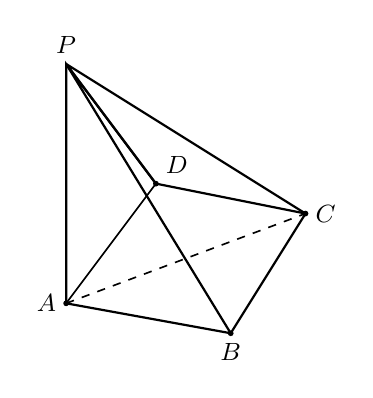
\begin{tikzpicture}[>=stealth, semithick, font=\small, scale=0.95]
  \coordinate (A) at (0,0);
  \coordinate (B) at (2.2,-0.4);
  \coordinate (D) at (1.2,1.6);
  \coordinate (C) at (3.2,1.2);
  \coordinate (P) at (0,3.2);
  \draw[thick] (P)--(A)--(B)--(C)--(D)--cycle;
  \draw[thick] (P)--(B) (P)--(C) (P)--(D);
  \draw[dashed] (A)--(C);
  \draw (A)--(D);
  \fill (A) circle (1.1pt) node[left] {$A$};
  \fill (B) circle (1.1pt) node[below] {$B$};
  \fill (C) circle (1.1pt) node[right] {$C$};
  \fill (D) circle (1.1pt) node[above right] {$D$};
  \node[above] at (P) {$P$};
\end{tikzpicture}
\end{center}
\nopagebreak[4]
\Needspace{4\baselineskip}
\textbf{解析}
\gksubpart{(1)}
$PA\perp$ 底面，故 $PA\perp AD$；又 $AB\perp AD$，故 $AD\perp$ 平面 $PAB$。而 $AD\subset$ 平面 $PAD$，故平面 $PAB\perp$ 平面 $PAD$。

\gksubpart{(2)}
\Needspace{5\baselineskip}
设 $A(0,0,0)$，$AB=m$，$AD=n$，$m+n=4$，$AP=m$。则
\nopagebreak[4]
\[B(m,0,0),\ D(0,n,0),\ P(0,0,m).\]
由 $CD=\sqrt2$、$\angle CDA=45^\circ$ 可取 $C(1,n-1,0)$。

\Needspace{5\baselineskip}
① 平面 $PCD$ 的法向量：$\overrightarrow{PC}=(1,n-1,-m)$，$\overrightarrow{PD}=(0,n,-m)$，
\nopagebreak[4]
\[\boldsymbol n=\overrightarrow{PC}\times\overrightarrow{PD}=(m,\,m,\,n).\]
\Needspace{5\baselineskip}
$\overrightarrow{PB}=(m,0,-m)$。由线面角 $30^\circ$：
\nopagebreak[4]
\[\sin30^\circ=\frac{|\overrightarrow{PB}\cdot\boldsymbol n|}{|\overrightarrow{PB}||\boldsymbol n|}
=\frac{m(m-n)}{m\sqrt2\sqrt{2m^2+n^2}}=\frac{|m-n|}{\sqrt2\sqrt{2m^2+n^2}}.\]
平方并代入 $n=4-m$，解得 $m=\dfrac45$。故 $AB=\dfrac45$。

\Needspace{5\baselineskip}
② 设 $G(0,t,0)$。由 $GP=GB$ 自动成立（$GP^2=t^2+m^2=GB^2$）。由 $GP=GD$：
\nopagebreak[4]
\[t^2+m^2=(n-t)^2\Longrightarrow t=\frac{n^2-m^2}{2n}.\]
\Needspace{5\baselineskip}
由 $GC=GD$：
\nopagebreak[4]
\[1+(n-1-t)^2=(n-t)^2\Longrightarrow t=n-1.\]
\Needspace{5\baselineskip}
联立得 $m^2+n^2-2n=0$，代入 $n=4-m$：
\nopagebreak[4]
\[2m^2-6m+8=0\Longrightarrow m^2-3m+4=0,\]
判别式 $9-16<0$，无实数解。故不存在这样的点 $G$。

\gkanswer{答案（1）：证明见解析。}

\gkanswer{答案（2）：① $AB=\dfrac45$；② 不存在。}

\end{answer}
\begin{answer}
\gksolhead{21}{}

\textbf{题目}：

三选二。

【A】设矩阵 $M=\begin{bmatrix}a&0\\0&b\end{bmatrix}$（其中 $a>0$，$b>0$）。

（1） 若 $a=2$，$b=3$，求矩阵 $M$ 的逆矩阵 $M^{-1}$；

（2） 若曲线 $C:x^2+y^2=1$ 在矩阵 $M$ 所对应的线性变换作用下得到曲线 $C':\dfrac{x^2}4+y^2=1$，求 $a$，$b$ 的值。

【B】在直角坐标系 $xOy$ 中，直线 $l$ 的方程为 $x-y+4=0$，曲线 $C$ 的参数方程为 $\begin{cases}x=\sqrt3\cos\alpha,\\y=\sin\alpha\end{cases}$（$\alpha$ 为参数）。

（1） 已知在极坐标中，点 $P$ 的极坐标为 $\left(4,\dfrac\pi2\right)$，判断点 $P$ 与直线 $l$ 的位置关系；

（2） 设点 $Q$ 是曲线 $C$ 上的一个动点，求它到直线 $l$ 的距离的最小值。

【C】设不等式 $|2x-1|<1$ 的解集为 $M$。

（1） 求集合 $M$；

（2） 若 $a$，$b\in M$，试比较 $ab+1$ 与 $a+b$ 的大小。

\Needspace{4\baselineskip}
\textbf{解析}
\gksubpart{(1)}
【A】 $M^{-1}=\begin{bmatrix}\frac12&0\\0&\frac13\end{bmatrix}$。
【B】 $P$ 的直角坐标为 $(0,4)$，代入 $x-y+4=0$ 得 $0-4+4=0$，故 $P$ 在 $l$ 上。
【C】 $|2x-1|<1\iff-1<2x-1<1\iff0<x<1$，故 $M=(0,1)$。

\gksubpart{(2)}
【A】 变换为 $x'=ax$，$y'=by$，圆变为 $\dfrac{x'^2}{a^2}+\dfrac{y'^2}{b^2}=1$，与 $\dfrac{x^2}4+y^2=1$ 比较得 $a=2$，$b=1$。
\Needspace{5\baselineskip}
【B】 点 $Q(\sqrt3\cos\alpha,\sin\alpha)$ 到 $l$ 的距离
\nopagebreak[4]
\[d=\frac{|\sqrt3\cos\alpha-\sin\alpha+4|}{\sqrt2}
=\frac{|2\cos(\alpha+\frac\pi6)+4|}{\sqrt2},\]
当 $\cos(\alpha+\frac\pi6)=-1$ 时最小，$d_{\min}=\sqrt2$。
【C】 $ab+1-(a+b)=(a-1)(b-1)$，因 $0<a,b<1$，故 $(a-1)(b-1)>0$，即 $ab+1>a+b$。

\gkanswer{答案（1）：A $M^{-1}=\begin{bmatrix}\frac12&0\\0&\frac13\end{bmatrix}$；B 点 $P$ 在直线 $l$ 上；C $M=(0,1)$。}

\gkanswer{答案（2）：A $a=2$，$b=1$；B 最小距离 $\sqrt2$；C $ab+1>a+b$。}

\end{answer}